% This is samplepaper.tex, a sample chapter demonstrating the
% LLNCS macro package for Springer Computer Science proceedings;
% Version 2.20 of 2017/10/04
%
\documentclass[runningheads]{llncs}
%
\usepackage{placeins}
\usepackage{amsmath}
\usepackage{graphicx}
\setcounter{MaxMatrixCols}{35}
% Used for displaying a sample figure. If possible, figure files should
% be included in EPS format.
%
% If you use the hyperref package, please uncomment the following line
% to display URLs in blue roman font according to Springer's eBook style:
% \renewcommand\UrlFont{\color{blue}\rmfamily}

\begin{document}
%
\title{Glamour or revulsion: A social analysis of HBO's Euphoria's influence on viewers' drug awareness and habits}%\thanks{Supported by organization x.}}
%
%\titlerunning{Abbreviated paper title}
% If the paper title is too long for the running head, you can set
% an abbreviated paper title here
%
\author{Maaz Saeed\inst{1}\orcidID{ms05050@st.habib.edu.pk} \and
Shayan Ahmed Shariff\inst{2,3}\orcidID{ss05582@st.habib.edu.pk} \and
Faiz Haseeb\inst{3}\orcidID{fh06224@st.habib.edu.pk}}
%
\authorrunning{M. Saeed et al.}
% First names are abbreviated in the running head.
% If there are more than two authors, 'et al.' is used.
%
\titlerunning{A social analysis of Euphoria's influence on viewers}
\institute{Habib University, Karachi Sindh 75290, Pakistan \\ \url{https://habib.edu.pk/}}
%
\maketitle              % typeset the header of the contribution
%
\begin{abstract}
In the contemporary world of competitive media, HBO had to bring something special to the table, more
than your average teenage-centered series. The hit television show boasts cinematography unmatched by
its competitors. From it’s drug-induced visuals, to it’s seamless transitions and imagery which is an ode to
famous art history. Consequently, the popularity invoked by such filming techniques has sparked
controversy and debate; the vibrant pictorial endeavour is often said to have glamorized the recreational
use of drugs with it’s narration of partying, sex, and rebellion. Our project aims to identify and study a friendship network, based on viewership of Euphoria. We
divided the people within the network into three subgroups: those who found their curiosity about a certain
drug(s) piqued, those who remained indifferent, and those who shied away from drug use, wary of the
dangers and risks portrayed by the show. From here onward, we analyzed the links in the
social network, examining the existence of characteristics such as peer pressure, social influence of popular
agents, not wanting to be isolated, in terms of of viewership within groups of friends;
phenomena such as triadic closures and clustering among members of the aforementioned subgroups; and
the nature of links between the three groups (for example, does the show bring together all viewers alike, or
are there bridges between different groups).

\keywords{Opinion Formation  \and Friendship Network \and Scale-Free Networks \and Drug Use \and Clustering }
\end{abstract}
%
%
%
\newpage

\section{Introduction}
In the contemporary post-modern world, we live in a society where opinions are no longer discussed merely during debates, but constantly as life goes on. Thanks to big data and the exponential growth of social media, came the sacrosanct infatuation to build a likable online presence, which further evolved into a need to maintain that presence even off-screens. As we move towards a smaller world each day, connections continue to be established, resulting in a massive flow of information, influence, and judgement.

Within this epoch of on-demand streaming, communication and opinion exertion, HBO came out with '\textit{Euphoria}'. In what is, perhaps, the biggest television series in the world today, the narration of events follows a group of teenagers battling with substance use (and abuse), climbing the social ladder, forming relationships, and then some.

In this paper our team set out to establish and analyze a friendship network among a university's student body, to examine the formation of links between individuals of similar and differing opinions; the only requirement being that they are viewers of Euphoria. 

\subsection{Methodology}
Our study aimed to collect data about viewership of Euphoria among the students of Habib University, both on an individual and friend group basis. We conducted an online survey to construct a cross-sectional representation of the student body and identify different characteristics embodied by the resulting friendship network, such as clustering and peer pressure.

This was done in two parts. The first part involved an online survey where students provided their reaction to the show from three possibilities: becoming averse towards drug use, being curious about a certain drug, or remaining indifferent. The second part involved respondents identifying their friends from among the other respondents. A total of 47 responses were received, out of which 34 were deemed usable. The reason for discarding some responses was either the lack of a response in the second part, or the student having zero friendship links to and from other students, which, since this study focuses primarily on friendship networks, is outside the scope of this paper, thus these isolates were left out of the final graph. 
\\

\section{Background and Scope}
To better study our findings, we primarily focused on some underlying foundations from social network analysis so that we may perceive our network from a few standard theorized properties such as:

\subsection{Triadic Closures}
Most networks are studied as a static structure at some instance of time. Though this is not an inaccurate measure, it is quite important to also view the potential evolution of a social network overtime.

Under the Strong Triadic Closure (STC) property if a node has a strong connection to two neighbours, those two neighbours will eventually form at least a weak connection between themselves [1].

In a social network, this link formation can be attributed to various factors such as wanting to increase one's social status by way of increasing their amount of friends, simply wanting to meet someone new, or among others, and by far the most likely, an organic blooming of friendship between the two due to being in the same room or part of the same conversation on numerous occasions due to their mutual friend.

\subsection{Structural Balance}
Structural balance is an intrinsic property of a network. One can conclude a network to be structurally-balanced if and only if all triads comprising the network on a graph are structurally-balanced, i.e. all triads have either only one positive dyad or all three positive dyads [2].

Since our survey did not probe respondents to present negative relationships, only positive ones, any and all links in our network are positive, and hence, we achieve structural balance.

\subsection{Clustering}
It often proves quite useful to group together elements of a network if they share certain characteristics. This enables easier identification and examination of patterns or structures that may be present within a population.  

This \textit{clustering analysis} may be carried out via measuring similarity using topology, i.e. location of nodes on a graph, the structure of the graph itself or type of node (assuming differing nodes are in place).

In our case, we can identify clusters by the location of nodes on the graph and how they are linked to their nearest neighbours, and by their view on drug use after viewership of the show.

\subsection{The Power Law Distribution}
A power law distribution is an exponential probability distribution, where changing one variable slightly produces a large change on the other variable. The distribution is characterized by the resulting graph being highly-skewed and asymmetric on a linear scale. The scalar relationship given by a power law can be represented by the following equation:
\[ p(x) = Cx^{-\alpha} \]

Where $\alpha$ is the power law exponent, and C is the normalization constant(needed as this is a probability distribution) [3]. 


\section{Literature Review and Application}
\subsection{Inspiration from previous works}
\subsubsection{Evolving structural balance}
Antal et al. in their paper, \textit{Social Balance on Networks: The Dynamics of Friendship and Enmity}, presented a dynamic phase transitioning of real-life social networks. They stated that an imbalanced graph can evolve into a balanced one, by the changing of relationships which ultimately alter the sign of a dyad. One of their proposed examples included a triad between a married couple and their friend; assuming a divorce taking place, the friend maintained a positive relationship with one member of the now ex-couple, and negated its relationship with the other [4]. Within this process there existed 3 different states of the graph: all positive links, two positive links, and eventually only one positive link. Intuitively, from structurally-balanced, to imbalanced, and back to balanced again.

Inspired by this example, we analyzed our friendship network and found triadic closures, as well as links from one common node(s) to a pair of non-linked nodes. Since our survey did not account for time, or changes in relationships, but merely the current relationship status of individuals, there is room for speculation insofar as perhaps not only is it possible for new friendships to bloom under the strong triadic closure property, but also the demise of previously existing friendships over difference of opinion. Granted that this assumption requires the acknowledgement of the fact that our network is only structurally balanced due to its pseudo nature of only depicting positive relationships and lack thereof, rather than also accounting for adversaries.

\subsubsection{Opinion formation of members of a network}
It is a widely accepted phenomena that individuals' tastes and opinions are often influenced by their peers. Altafini claimed that if a major feature of structurally-balanced networks is that the decisions arrived at by members of a community are influenced by the social networks they belong to, then among the properties of such a system are some borrowed from monotone dynamics [5]. Further, in monotone systems, the initially seeded idea is likely to boast a competitive advantage over ones that follow [5]. 

For a real-life social network, we can attribute this competitive advantage to factors such popularity and, / or peer pressure. It is natural for an individual to be inclined towards agreeing with an agent of immense popularity, even if they may not wholeheartedly share a belief. It is also entirely possible for opinions to change overtime due to fear of isolation (feeling left out). 

In the previous section, 3.1, we have discussed the structural balance of our friendship network. Just as the strong triadic closure property states that a link will eventually form between two nodes who share a strong link with a mutual node, coupled with the aforementioned social reasons, we believe it is highly likely for an already existing triad, where two members are of a common opinion, to (either directly, or indirectly) persuade the third member to reevaluate their opinion on the recreational use of drugs; similar to Altafini's example of two-faction political political coalition, where it is an either-or decision with a clear distinction between the two sides.

\subsubsection{Power Laws and Scale-Free Networks}
Barabasi differentiates networks that follow a power law distribution from those that follow a Poisson distribution more typical of random networks than real-world networks. He defines these "scale-free" networks as follows: \textit{A scale-free network is a network whose degree distribution follows a power
law} [6].

Since our study aims to analyse a friendship network, it is pertinent here to include the following example from Barabasi's book on real world scale-free networks that shows the degree distribution of a scale-free network plotted out in graph form, to illustrate what we expect the degree distribution of our network to look like (see Fig.~\ref{fig1}).
\begin{figure}
\begin{center}
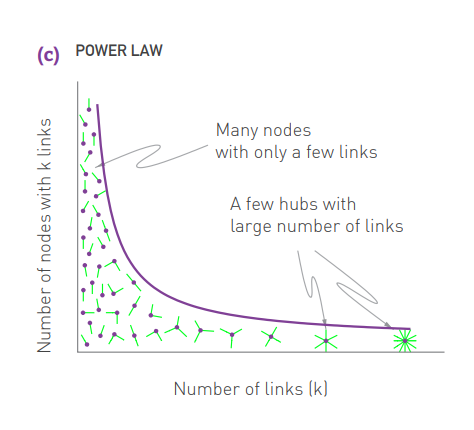
\includegraphics[width=0.7\textwidth]{Project/barabasi.png}
\caption{The degree distribution of a scale-free network follows a power law [6].} \label{fig1}
\end{center}
\end{figure}
\FloatBarrier

\newpage
\subsection{Our Findings}
\subsubsection{Responses}
The responses were almost completely uniformly distributed among the three options for reactions to the show, with being influenced to shy away from using drugs having only one more response than the other two choices (see Fig.~\ref{fig2}).
\begin{figure}
\begin{center}
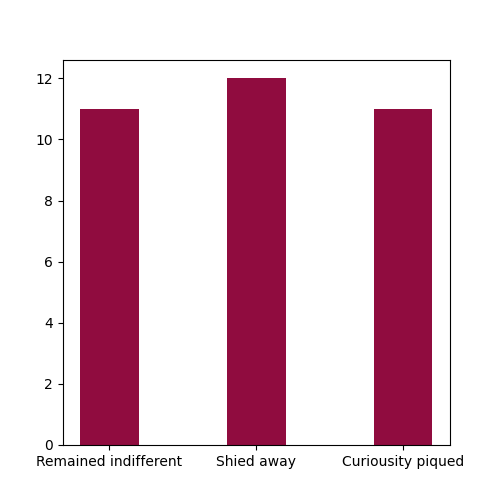
\includegraphics[width=0.7\textwidth]{Project/fig2.png}
\caption{Distribution of responses.} \label{fig2}
\end{center}
\end{figure}
\FloatBarrier
As we can see, there is no clear bias towards one reaction to the show over the other. The respondents are distributed evenly across all three possible responses to viewing the show, which can be stated to be an argument for the show not particularly influencing students' attitudes towards drug use in one direction or the other as part of a general trend, but at this stage it is too early to draw a conclusive answer. The responses were compiled into a graph using the NetworkX library in python in order to perform further analysis. 

However, although the responses are not skewed in one particular direction, a significant portion of the population was influenced to have a strong reaction one way or the other, being drawn towards or away from the idea of drug use. The people who remained indifferent are about half of the sum of the two who were influenced in some way, and so the respondents who remained indifferent make up a minority of the overall population, so it can be said that the show has a significant impact on viewers' perception of drugs and drug use.
\subsubsection{Results}
The resulting network consists of a large, dense, highly clustered central friend group, with individual students from this super-group having links to students on the periphery. These results are presented as a graph with nodes being students, and edges being friendship links (see Fig.~\ref{fig3}).

\begin{figure}
\begin{center}
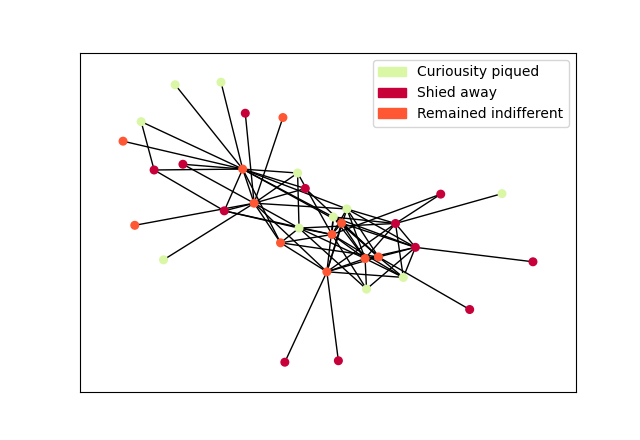
\includegraphics[width=0.8\textwidth]{Project/fig3.png}
\caption{Visualisation of the Euphoria friendship network.} \label{fig3}
\end{center}
\end{figure}
\FloatBarrier
The results show that most people who responded to the survey are part of one large, highly-connected friend group, with some outliers on the periphery. What is interesting to note is that the majority of the respondents that remained indifferent or had their curiosity piqued after watching the show have a high degree, i.e they are very popular individuals. Meanwhile, most of those who were turned off from drugs after watching the show are on the very fringe, or close to the fringe. The adjacency matrix representation of this network is given in the appendix (see Fig.~\ref{fig5}).

We believe this illustrates the extent to which drug use, or at least the aesthetic of drug use has been normalized in adolescents. Shying away from drugs correlates with being more isolated, while being curious correlates with being more popular. Ambivalence also correlating with popularity could be in part attributed to people without strong opinions in either direction being more easy to get along with. The curious group being more popular could also be in part due to these individuals being more willing to try new things or them being less risk-averse, which would give them the advantage in a social setting. Follow up research needs to be conducted in this regard. 

\subsubsection{Degree Analysis} 
We can plot the degree distribution of this network in a histogram as follows (see Fig.~\ref{fig4}).

\begin{figure}
\begin{center}
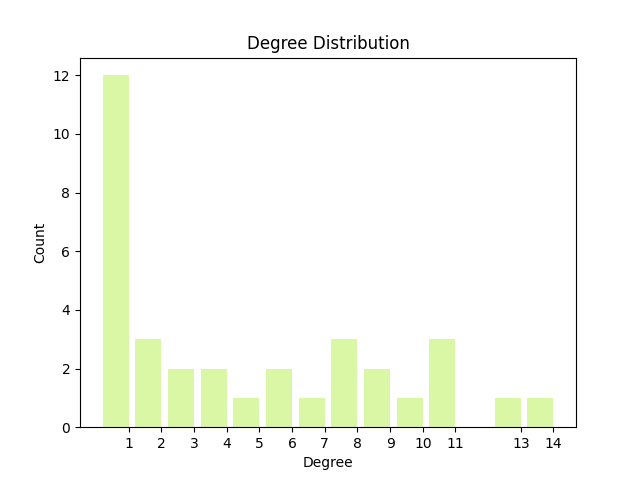
\includegraphics[width=0.8\textwidth]{Project/fig4.png}
\caption{Frequency of node degree in the Euphoria friendship network} \label{fig4}
\end{center}
\end{figure}
\FloatBarrier
Though our sample size is too small to tell for sure, if we look back at Fig 1, and compare the two, our network appears to loosely follow a power law distribution. We see the vast majority of nodes have a degree of 1, and then the degree frequency drops off into a heavy tail. There are some outliers but this can be explained by the limited number of responses at our disposal. Further work can be done here, for example a repeat of the survey with a much larger sample size, in order to make a more confident assertion about if friendship networks in the university follow a power law distribution.


\section{Contextualization}
\subsection{Growing prevalence of drugs in Pakistani Media}
We cannot begin to discuss the impact of Euphoria on the perception of drugs and drug use without also analyzing the general view of substance use in young adults in Pakistani society. We see the use of drugs normalised amongst Pakistani musical artists for one. From Faris Shafi smoking a marijuana joint in the music video for his song Molotov [7], to Talha Yunus sitting surrounded by kilos of the same (be it props) in the video for Young Stunners' Quarantine [8], one cannot deny the normalisation of drugs in our culture, and the fact that movies, television shows, and music videos have an effect on the youth of Pakistan. Depending on person to person, this effect varies, as shown in our study. Moreover, our study does indicate the normalisation of recreational drugs in social networks, as those whose interest grew by watching Euphoria seem to have a higher degree centrality, meaning they are well connected.

\subsection{Previous studies on adolescent population of Pakistan indulging in substance use}
Further developing on the influence on young adults in Pakistan, to begin using drugs, peer pressure is also a significant factor. In a study conducted in 2012 by the Department of Rural Sociology in the University of Agriculture in Faisalabad [9], 500 addicts in five government rehabilitation centers in Punjab hospitals were given a questionnaire and interviewed. In the questionnaire, they were asked if various factors contributed to their drug use, of which one was peer pressure. 68\% of the addicts agreed that it affected their drug use to a great extent. This data again speaks to the level of normalisation that drug use has in friend groups, which our data displays, and while people may not be forcibly pressuring their friends to try drugs, one is certainly more likely to try them if a large proportion of their friends are.

\subsection{Sense of belonging rationalized by relating to characters on-screen}
It is also important to consider how the characters of Euphoria are not perfect, but portrayed as quite relatable. In the show, many characters struggle with trauma due to their parents. Rue, the main character, begins using drugs to cope with the loss of her father to cancer. Cassie, another character, alongside her sister and mother, is abandoned at a young age by her father, who is also an addict. She grows up to develop a drinking problem insofar as she is not an addict but can not limit herself when she does indulge in consumption of alcohol. 

The aforementioned study also presents parental problems, namely neglect, as one of the reasons people abuse drugs, with 60\% of the participants admitting it played some part in their addiction. In addition to this, the study also cites loneliness, as a result of the loss of a companion, spouse, or parent as a reason for drug abuse, with 67\% of all addicts agreeing that it played some part. This is another theme explored by the show, where Maddie turns to the party drug 'Molly' after dissension with her boyfriend Nate. People who have little to no parental guidance or who have experienced great loss in relationships will often turn to drugs as a way to fulfil this emotional deficiency, which is what Euphoria depicts, and is what people watching it relate to.

Viewers of the show suffering from similar problems will find comfort in the knowledge that other people experience the same things, and that these seemingly harmful choices they choose to make, are not a self-exile from society but perhaps a more, unspoken, truth of being human. And so, will replicate these coping mechanisms that the characters in the show use, attracted by the glamour of the highs. Or be revolted by the lows of addiction, and the fear of going off the deep-end, to inevitably experience the same social, physical, and lawful consequences faced by some of the characters.

\section{Appendix}
\subsection{Adjacency Matrix}
\begin{figure}
\[\begin{pmatrix}
0 & 1 & 1 & 1 & 1 & 1 & 0 & 0 & 1 & 0 & 0 & 1 & 0 & 0 & 1 & 0 & 0 & 0 & 0 & 0 & 1 & 0 & 0 & 0 & 1 & 0 & 0 & 0 & 0 & 0 & 0 & 0 & 0 & 0 \\
1 & 0 & 1 & 1 & 1 & 0 & 0 & 1 & 1 & 1 & 0 & 0 & 0 & 0 & 0 & 0 & 0 & 0 & 0 & 0 & 0 & 0 & 0 & 0 & 0 & 0 & 1 & 0 & 0 & 0 & 0 & 0 & 0 & 0 \\
1 & 1 & 0 & 1 & 0 & 1 & 0 & 0 & 1 & 1 & 0 & 0 & 0 & 0 & 0 & 1 & 0 & 0 & 0 & 0 & 1 & 1 & 0 & 0 & 1 & 1 & 0 & 0 & 0 & 0 & 0 & 0 & 0 & 0 \\
1 & 1 & 1 & 0 & 1 & 1 & 0 & 1 & 1 & 1 & 1 & 0 & 0 & 0 & 0 & 0 & 0 & 0 & 0 & 0 & 1 & 0 & 1 & 0 & 0 & 0 & 0 & 0 & 0 & 0 & 0 & 0 & 0 & 0 \\
1 & 1 & 0 & 1 & 0 & 1 & 1 & 0 & 1 & 1 & 0 & 0 & 0 & 0 & 0 & 0 & 0 & 0 & 0 & 0 & 1 & 0 & 1 & 0 & 0 & 0 & 0 & 0 & 0 & 0 & 0 & 0 & 0 & 0 \\
1 & 0 & 1 & 1 & 1 & 0 & 0 & 1 & 0 & 1 & 0 & 0 & 0 & 0 & 0 & 0 & 0 & 0 & 0 & 0 & 0 & 0 & 0 & 0 & 0 & 0 & 0 & 0 & 0 & 0 & 0 & 0 & 0 & 0 \\
0 & 0 & 0 & 0 & 1 & 0 & 0 & 0 & 0 & 0 & 0 & 0 & 0 & 0 & 0 & 0 & 0 & 0 & 0 & 0 & 0 & 0 & 0 & 0 & 0 & 0 & 0 & 0 & 0 & 0 & 0 & 0 & 0 & 0 \\
0 & 1 & 0 & 1 & 0 & 1 & 0 & 0 & 1 & 0 & 1 & 0 & 0 & 0 & 0 & 0 & 0 & 0 & 1 & 0 & 1 & 0 & 1 & 0 & 1 & 0 & 0 & 1 & 0 & 1 & 0 & 0 & 0 & 0 \\
1 & 1 & 1 & 1 & 1 & 0 & 0 & 1 & 0 & 0 & 0 & 0 & 0 & 0 & 0 & 0 & 0 & 0 & 0 & 0 & 0 & 0 & 0 & 0 & 0 & 0 & 1 & 0 & 0 & 0 & 0 & 0 & 0 & 0 \\
0 & 1 & 1 & 1 & 1 & 1 & 0 & 0 & 0 & 0 & 1 & 0 & 0 & 0 & 0 & 0 & 0 & 0 & 0 & 0 & 1 & 0 & 0 & 0 & 0 & 0 & 0 & 1 & 0 & 0 & 0 & 0 & 0 & 1 \\
0 & 0 & 0 & 1 & 0 & 0 & 0 & 1 & 0 & 1 & 0 & 0 & 0 & 0 & 0 & 0 & 0 & 0 & 1 & 0 & 0 & 0 & 1 & 0 & 1 & 1 & 0 & 0 & 0 & 1 & 0 & 0 & 0 & 0 \\
1 & 0 & 0 & 0 & 0 & 0 & 0 & 0 & 0 & 0 & 0 & 0 & 0 & 0 & 0 & 0 & 0 & 0 & 0 & 0 & 0 & 0 & 0 & 0 & 0 & 1 & 1 & 0 & 0 & 0 & 0 & 0 & 0 & 0 \\
0 & 0 & 0 & 0 & 0 & 0 & 0 & 0 & 0 & 0 & 0 & 0 & 0 & 0 & 0 & 0 & 0 & 0 & 0 & 0 & 0 & 0 & 0 & 0 & 0 & 1 & 0 & 0 & 0 & 0 & 0 & 0 & 0 & 0 \\
0 & 0 & 0 & 0 & 0 & 0 & 0 & 0 & 0 & 0 & 0 & 0 & 0 & 0 & 0 & 0 & 0 & 0 & 0 & 0 & 0 & 0 & 0 & 0 & 0 & 1 & 0 & 0 & 0 & 0 & 0 & 0 & 0 & 0 \\
1 & 0 & 0 & 0 & 0 & 0 & 0 & 0 & 0 & 0 & 0 & 0 & 0 & 0 & 0 & 0 & 0 & 0 & 0 & 0 & 0 & 0 & 0 & 0 & 0 & 0 & 0 & 0 & 0 & 0 & 0 & 0 & 0 & 0 \\
0 & 0 & 1 & 0 & 0 & 0 & 0 & 0 & 0 & 0 & 0 & 0 & 0 & 0 & 0 & 0 & 0 & 0 & 0 & 0 & 0 & 0 & 0 & 0 & 0 & 0 & 0 & 0 & 0 & 0 & 0 & 0 & 0 & 0 \\
0 & 0 & 0 & 0 & 0 & 0 & 0 & 0 & 0 & 0 & 0 & 0 & 0 & 0 & 0 & 0 & 0 & 0 & 0 & 0 & 0 & 0 & 0 & 0 & 0 & 0 & 1 & 0 & 0 & 0 & 0 & 0 & 0 & 0 \\
0 & 0 & 0 & 0 & 0 & 0 & 0 & 0 & 0 & 0 & 0 & 0 & 0 & 0 & 0 & 0 & 0 & 0 & 0 & 0 & 0 & 0 & 0 & 0 & 0 & 0 & 1 & 0 & 0 & 0 & 0 & 0 & 0 & 0 \\
0 & 0 & 0 & 0 & 0 & 0 & 0 & 1 & 0 & 0 & 1 & 0 & 0 & 0 & 0 & 0 & 0 & 0 & 0 & 0 & 0 & 0 & 0 & 0 & 0 & 1 & 1 & 0 & 0 & 0 & 0 & 0 & 0 & 0 \\
0 & 0 & 0 & 0 & 0 & 0 & 0 & 0 & 0 & 0 & 0 & 0 & 0 & 0 & 0 & 0 & 0 & 0 & 0 & 0 & 0 & 0 & 0 & 0 & 0 & 1 & 1 & 0 & 0 & 0 & 0 & 0 & 0 & 0 \\
1 & 0 & 1 & 1 & 1 & 0 & 0 & 1 & 0 & 1 & 0 & 0 & 0 & 0 & 0 & 0 & 0 & 0 & 0 & 0 & 0 & 0 & 0 & 0 & 0 & 1 & 1 & 0 & 0 & 0 & 0 & 0 & 0 & 0 \\
0 & 0 & 1 & 0 & 0 & 0 & 0 & 0 & 0 & 0 & 0 & 0 & 0 & 0 & 0 & 0 & 0 & 0 & 0 & 0 & 0 & 0 & 0 & 0 & 0 & 0 & 0 & 0 & 0 & 0 & 0 & 0 & 0 & 0 \\
0 & 0 & 0 & 1 & 1 & 0 & 0 & 1 & 0 & 0 & 1 & 0 & 0 & 0 & 0 & 0 & 0 & 0 & 0 & 0 & 0 & 0 & 0 & 0 & 0 & 0 & 0 & 0 & 0 & 0 & 0 & 0 & 0 & 0 \\
0 & 0 & 0 & 0 & 0 & 0 & 0 & 0 & 0 & 0 & 0 & 0 & 0 & 0 & 0 & 0 & 0 & 0 & 0 & 0 & 0 & 0 & 0 & 0 & 0 & 1 & 0 & 0 & 0 & 0 & 0 & 0 & 0 & 0 \\
1 & 0 & 1 & 0 & 0 & 0 & 0 & 1 & 0 & 0 & 1 & 0 & 0 & 0 & 0 & 0 & 0 & 0 & 0 & 0 & 0 & 0 & 0 & 0 & 0 & 1 & 1 & 0 & 0 & 0 & 0 & 0 & 0 & 0 \\
0 & 0 & 1 & 0 & 0 & 0 & 0 & 0 & 0 & 0 & 1 & 1 & 1 & 1 & 0 & 0 & 0 & 0 & 1 & 1 & 1 & 0 & 0 & 1 & 1 & 0 & 1 & 0 & 0 & 1 & 0 & 1 & 0 & 0 \\
0 & 1 & 0 & 0 & 0 & 0 & 0 & 0 & 1 & 0 & 0 & 1 & 0 & 0 & 0 & 0 & 1 & 1 & 1 & 1 & 1 & 0 & 0 & 0 & 1 & 1 & 0 & 0 & 1 & 1 & 1 & 0 & 1 & 0 \\
0 & 0 & 0 & 0 & 0 & 0 & 0 & 1 & 0 & 1 & 0 & 0 & 0 & 0 & 0 & 0 & 0 & 0 & 0 & 0 & 0 & 0 & 0 & 0 & 0 & 0 & 0 & 0 & 0 & 0 & 0 & 0 & 0 & 0 \\
0 & 0 & 0 & 0 & 0 & 0 & 0 & 0 & 0 & 0 & 0 & 0 & 0 & 0 & 0 & 0 & 0 & 0 & 0 & 0 & 0 & 0 & 0 & 0 & 0 & 0 & 1 & 0 & 0 & 0 & 0 & 0 & 1 & 0 \\
0 & 0 & 0 & 0 & 0 & 0 & 0 & 1 & 0 & 0 & 1 & 0 & 0 & 0 & 0 & 0 & 0 & 0 & 0 & 0 & 0 & 0 & 0 & 0 & 0 & 1 & 1 & 0 & 0 & 0 & 0 & 0 & 1 & 0 \\
0 & 0 & 0 & 0 & 0 & 0 & 0 & 0 & 0 & 0 & 0 & 0 & 0 & 0 & 0 & 0 & 0 & 0 & 0 & 0 & 0 & 0 & 0 & 0 & 0 & 0 & 1 & 0 & 0 & 0 & 0 & 0 & 0 & 0 \\
0 & 0 & 0 & 0 & 0 & 0 & 0 & 0 & 0 & 0 & 0 & 0 & 0 & 0 & 0 & 0 & 0 & 0 & 0 & 0 & 0 & 0 & 0 & 0 & 0 & 1 & 0 & 0 & 0 & 0 & 0 & 0 & 0 & 0 \\
0 & 0 & 0 & 0 & 0 & 0 & 0 & 0 & 0 & 0 & 0 & 0 & 0 & 0 & 0 & 0 & 0 & 0 & 0 & 0 & 0 & 0 & 0 & 0 & 0 & 0 & 1 & 0 & 1 & 1 & 0 & 0 & 0 & 0 \\
0 & 0 & 0 & 0 & 0 & 0 & 0 & 0 & 0 & 1 & 0 & 0 & 0 & 0 & 0 & 0 & 0 & 0 & 0 & 0 & 0 & 0 & 0 & 0 & 0 & 0 & 0 & 0 & 0 & 0 & 0 & 0 & 0 & 0
\end{pmatrix}\]
\caption{Adjacency Matrix representation of the Euphoria friendship network} \label{fig5}
\end{figure}
\FloatBarrier
\section{}


\begin{thebibliography}{8}
%\bibitem{ref_article1}
%Author, F.: Article title. Journal \textbf{2}(5), 99--110 %(2016)

%\bibitem{ref_lncs1}
%Author, F., Author, S.: Title of a proceedings paper. In: %Editor,
%F., Editor, S. (eds.) CONFERENCE 2016, LNCS, vol. 9999, pp. %1--13.
%Springer, Heidelberg (2016). \doi{10.10007/1234567890}

%\bibitem{ref_book1}
%Author, F., Author, S., Author, T.: Book title. 2nd edn. %Publisher,
%Location (1999)

%\bibitem{ref_proc1}
%Author, A.-B.: Contribution title. In: 9th International %Proceedings
%on Proceedings, pp. 1--2. Publisher, Location (2010)

%\bibitem{ref_url1}
%LNCS Homepage, \url{http://www.springer.com/lncs}. Last accessed 4
%Oct 2017

%samples refs end here, real ones begin

%1
\bibitem{stc}
Easly, D., Kleinberg, J.: Networks, Crowds, and Markets: Reasoning about a Highly Connected World. 1st edn. Cambridge University Press,
Cambridge (2010)

%2
\bibitem{stbal}
Alam, S.J.: CS 363 - Week 09 - The Structural Balance Theory - Spring 2022. (2022). 

%3
\bibitem{pwrlaw}
Alam, S.J.: CS 363 - Week 07 - An Introduction to Power-Laws - Spring 2022. (2022). 

%4
\bibitem{st_evo}
Antal, T., Krapivsky, P.L., Redner, S.: Social Balance on networks: The dynamics of friendship and enmity. Physica D: Nonlinear Phenomena. 224, 130–136 (2006).
\doi{10.1016/j.physd.2006.09.028}

%5
\bibitem{opinion}
Altafini, C.: Dynamics of Opinion Forming in Structurally Balanced Social Networks. PLoS ONE 7(6): e38135., (2012) https://doi.org/10.1371/journal.pone.0038135

%6
\bibitem{barabasi}
Barabási, A.: Network science. Cambridge University Press, Cambridge (2016).

%7
\bibitem{faris}
Parvez, A.M., Qureshi, T., Gohar, A.: Molotov. YouTube (2021). 

%8
\bibitem{quarantine}
Anjum, T., Yunus, T., Hameed, N.: QUARANTINE. YouTube (2020). 

%9
\bibitem{pak_drugs}
Siddique, F., Mann, A.A., Ali, T.: Influence of social factors on drug use behavior in Punjab, Pakistan. Pakistan Journal of Nutrition. 11, 1099–1100 (2012). 
\end{thebibliography}
\end{document}
